\documentclass{sig-alternate}

\usepackage{times}
\usepackage{url}
\usepackage{todonotes}
\sloppy

\setlength{\parindent}{0.5cm} 

\newcommand{\citep}[1]{\cite{#1}}

% Copyright
\setcopyright{acmcopyright}
%\setcopyright{acmlicensed}
%\setcopyright{rightsretained}
%\setcopyright{usgov}
%\setcopyright{usgovmixed}
%\setcopyright{cagov}
%\setcopyright{cagovmixed}


% DOI
\doi{10.475/123_4}

% ISBN
\isbn{123-4567-24-567/08/06}

\acmPrice{\$15.00}

% You need the command \numberofauthors to handle the 'placement
% and alignment' of the authors beneath the title.
%
% For aesthetic reasons, we recommend 'three authors at a time'
% i.e. three 'name/affiliation blocks' be placed beneath the title.
%
% NOTE: You are NOT restricted in how many 'rows' of
% "name/affiliations" may appear. We just ask that you restrict
% the number of 'columns' to three.
%
% Because of the available 'opening page real-estate'
% we ask you to refrain from putting more than six authors
% (two rows with three columns) beneath the article title.
% More than six makes the first-page appear very cluttered indeed.
%
% Use the \alignauthor commands to handle the names
% and affiliations for an 'aesthetic maximum' of six authors.
% Add names, affiliations, addresses for
% the seventh etc. author(s) as the argument for the
% \additionalauthors command.
% These 'additional authors' will be output/set for you
% without further effort on your part as the last section in
% the body of your article BEFORE References or any Appendices.

\begin{document}

\conferenceinfo{GECCO'16,} {July 20-24, 2016, Denver, Colorado, USA.}
\CopyrightYear{2016}
\crdata{TBA}
\clubpenalty=10000
\widowpenalty = 10000

\title{Visualizing genetic programming ancestries using graph databases}

%\numberofauthors{5}
%\author{
%\alignauthor
%Nicholas Freitag McPhee\\
%	\affaddr{Div. of Science and Math}\\
%	\affaddr{Univ. of Minnesota, Morris}\\
%	\affaddr{Morris, MN USA-56267}\\
%	\email{mcphee@morris.umn.edu}
%\alignauthor
%Maggie M. Casale\\
%	\affaddr{Div. of Science and Math}\\
%	\affaddr{Univ. of Minnesota, Morris}\\
%	\affaddr{Morris, MN USA-56267}\\
%	\email{casal033@morris.umn.edu}
%\alignauthor
%Mitchell Finzel \\
%	\affaddr{Div. of Science and Math}\\
%	\affaddr{Univ. of Minnesota, Morris}\\
%	\affaddr{Morris, MN USA-56267}\\
%	\email{finze008@morris.umn.edu}
%\and
%\alignauthor
%Thomas Helmuth\\
%	\affaddr{Computer Science Dep't}\\
%	\affaddr{Washington and Lee Univ.}\\
%	\affaddr{Lexington, VA USA-24450}\\
%	\email{helmutht@wlu.edu}
%\alignauthor
%Lee Spector\\
%	\affaddr{Cognitive Science}\\
%	\affaddr{Hampshire College}\\
%	\affaddr{Amherst, MA USA-01002}\\
%	\email{lspector@hampshire.edu}
%}

\maketitle

\begin{abstract}

Previous work has demonstrated the utility of graph databases as a tool 
for collecting, analyzing, and visualizing ancestry in evolutionary computation runs. 
That work focused on sections of individual runs, whereas this paper 
illustrates the application of these ideas on the entirety of large runs 
(up to three hundred thousand individuals) and combinations of multiple runs.

Here we use these tools to generate graphs showing \emph{all} the 
ancestors of successful individuals from a variety of stack-based 
genetic programming runs on software synthesis problems. These graphs 
highlight important moments in the evolutionary process. They also 
allow us to compare the dynamics when using different evolutionary tools, 
such as the dynamics for successful and unsuccessful runs.

As well as displaying these full ancestry graphs, we use a
variety of standard techniques such as size, color, pattern,
labeling, and opacity to visualize other important information such as fitness, 
which genetic operators were used, and the distance between parent and
child genomes. While this generates an extremely rich visualization,
the amount of data can also be somewhat overwhelming, so we also
explore techniques for filtering these graphs that allow us to better
understand the key dynamics.

\end{abstract}

\begin{CCSXML}
	<ccs2012>
	<concept>
	<concept_id>10003120.10003145.10003146.10010892</concept_id>
	<concept_desc>Human-centered computing~Graph drawings</concept_desc>
	<concept_significance>500</concept_significance>
	</concept>
	<concept>
	<concept_id>10003120.10003145.10003147.10010364</concept_id>

	<concept_desc>Human-centered computing~Scientific visualization</concept_desc>
	<concept_significance>500</concept_significance>
	</concept>
	<concept>
	<concept_id>10010147.10010178.10010205.10010206</concept_id>
	<concept_desc>Computing methodologies~Heuristic function construction</concept_desc>
	<concept_significance>300</concept_significance>
	</concept>
	<concept>
	<concept_id>10010147.10010257.10010293.10011809.10011813</concept_id>
	<concept_desc>Computing methodologies~Genetic programming</concept_desc>
	<concept_significance>300</concept_significance>
	</concept>
	</ccs2012>
\end{CCSXML}

\ccsdesc[500]{Human-centered computing~Graph drawings}
\ccsdesc[500]{Human-centered computing~Scientific visualization}
\ccsdesc[300]{Computing methodologies~Heuristic function construction}
\ccsdesc[300]{Computing methodologies~Genetic programming}

\printccsdesc

\keywords{visualization; genetic programming; graph database; ancestry}

\section{Introduction}
\label{sec:introduction}

Our reporting of results in genetic programming (GP) and evolutionary computation 
is frequently limited to aggregate statistics such as mean best fitness or 
percentage of successful runs. Unfortunately this fails to convey the complex 
dynamics of such evolutionary systems and obscures or omits potentially valuable 
information about \emph{why} the runs behaved as they did. While it's clearly
valuable to know that Approach A is ``better'' in some sense (e.g., more successes)
than Approach B, it is also valuable to understand \emph{why} it succeeds more 
often, a question that summary statistics rarely shed any light on.

One way to move past the limitations of summary statistics is to collect ancestry
information on runs, recording and analyzing parent--child 
relationships~\cite{burlacu2013visualization,cruz2015elicit,hart2001gavel,vaseux2013event}. \
Most previous ancestry
work has been limited to fairly small datasets, however, in part because of the
challenges of storing and working effectively with the hundreds of thousands of
ancestry relationships present in most evolutionary computation runs.

Previous work~\cite{McPhee:2015:GPTP} has demonstrated the utility of graph databases as 
tools for collecting and analyzing large collections of ancestry data from GP runs,
helping to identify key moments in runs, and general behavioral trends. That work,
however, was focused on sections of individual runs. In this paper we illustrate the 
use of these tools as a means of visualizing and exploring entire 
ancestry trees, and combinations of ancestry trees. 
We use the Titan graph database\footnote{\url{http://
thinkaurelius.github.io/titan/}} along with the Gremlin shell and the Tinkerpop query 
tools\footnote{\url{https://tinkerpop.apache.org/}} to store the parent-child 
relationships from genetic programming runs, and to extract the ancestry trees of 
specified individuals. We then visualize these subgraphs using the Graphviz \texttt{dot} 
graph layout tool.\footnote{\url{http://www.graphviz.org/}}

In the next section (Section~\ref{sec:testEnv}) we will describe the test
environment used to generate the data used in this paper. Section~\ref{sec:basics}
describes the basic graph structure used in these visualizations, including
detailed descriptions of how the rendering of edges and nodes conveys additional
information about the individuals and run dynamics. The initial graphs are large
enough to be rather overwhelming, so in Section~\ref{sec:filtering} we describe
ways to filter these large graphs into more comprehensible subgraphs. 
Section~\ref{sec:comparisons} provides examples of our ability to compare multiple
runs side-by-side, illustrating similarities and differences in the run dynamics.
We wrap up with some ideas for future work in Section~\ref{sec:futurework} and
conclusions in Section~\ref{sec:conclusions}.

\section{Our test environment: PushGP \& Replace Space With Newline}
\label{sec:testEnv}

All the visualizations presented here are on runs using the Clojush
implementation\footnote{\url{https://github.com/lspector/Clojush}} of the 
PushGP genetic programming (GP) system~\cite{1068292,spector:2002:GPEM}, 
but all of the ideas here
could easily apply to almost any evolutionary computation system. The use
of graph databases to capture ancestor lineage is a completely general
concept, for example, and could be applied to any system that implements a
notion of descent with modification. Some of the specifics of the visualization
are tied to particular metrics (e.g., the Damerau--Levenshtein distance
between Push program genomes), but these could be replaced with other
metrics as appropriate to the application domain (e.g., manhattan distances
between genetic algorithms bitstrings, or tree edit distances in
tree-based GP).

One important feature of the PushGP system is the use of \emph{lexicase
selection}~\cite{Helmuth:2015:ieeeTEC}. One of the goals in the design of
lexicase selection was the preservation of diversity of behaviors. The
ancestry information in the graph databases and in the tree visualizations 
in this paper can be used to visually and quantitatively check how
well those goals are being met. One property of lexicase selection is
that it enables the possibility of \emph{hyperselection} events~\cite{Helmuth:2016:GECCO},
where an individual receives an extremely high proportion of the selections
in a given generation. Occasionally, for example, an individual that
"discovers" an important new behavior can receive over 90\% of the selections
and consequently be a parent of nearly all the children in the next generation.
These hyperselection events will be visually obvious in our graph visualizations
below.

We have applied the visualizations described here on a 
number of different problems taken from a suite of software synthesis benchmark 
problems~\cite{Helmuth:2015:GECCO}, but in the interest of space we
will focus here on a single test problem: Replace Space With Newline.
In Replace Space With Newline the goal is to evolve a program that takes a string
as input and has two tasks: (a) it should print the input string, with all spaces
replaced by newlines, and (b) it should return an integer that is the number of
characters in the input string that were \emph{not} replaced. The use of
these two distinct types of error values will be used in some of the visualizations
as described in Section~\ref{sec:nodes}. 

The details of the system and settings used in these runs are as described 
in~\cite{Helmuth:2015:GECCO}. There are, however, two parameters that are 
directly relevant to these visualizations: The population size was 1,000, and the runs were stopped after 300 generations if a successful individual was not 
found. This means that we were storing and processing considerable information
on up to 300,000 individuals.

\section{Basic Graph Structure}
\label{sec:basics}

\begin{figure}[b]
	\begin{center}
		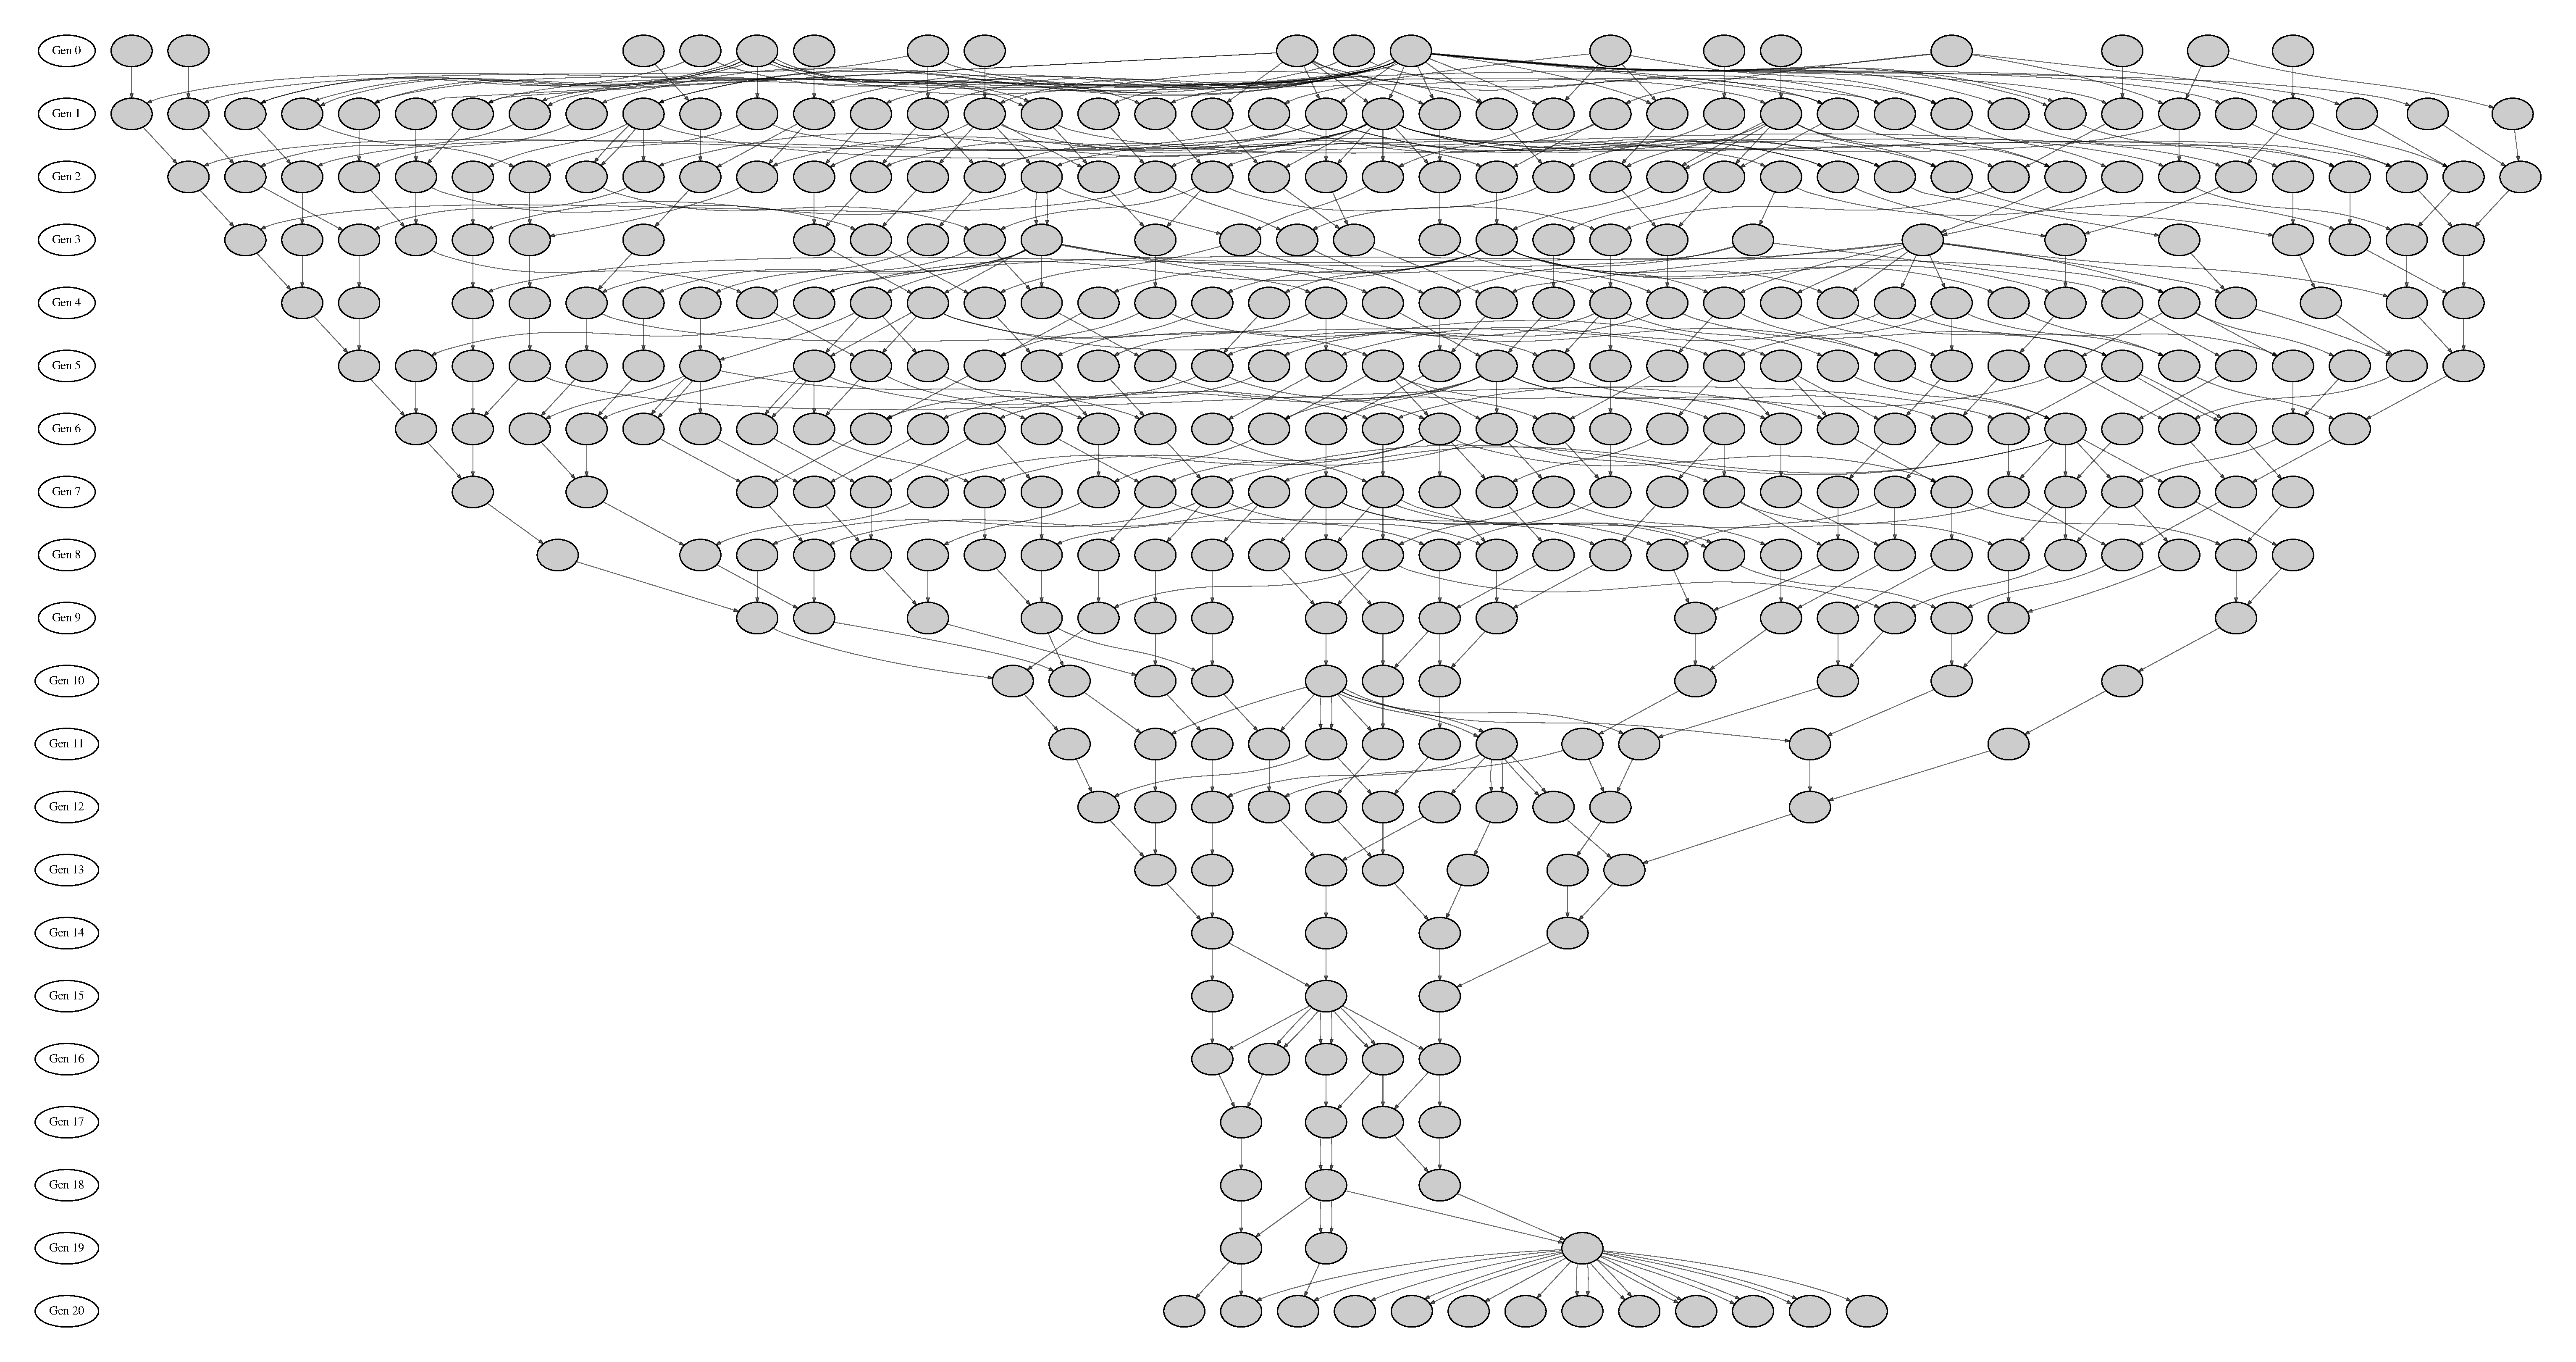
\includegraphics[width=\linewidth]{../Figures/run0_basic_structure.pdf}
	\end{center}
	\caption{Basic layout of ancestry trees, showing parent-child relationships. Generations are labeled on the left-hand side.}
	\label{fig:lexRun0Basic}
\end{figure}

These evolutionary computation runs are shown in the form of their ancestry trees. For a successful run, where at least one individual has found a solution to the problem, we get the ancestry tree by finding all individuals who have found a solution in the final generation. With these individuals, we go back through generations to retrieve their parents, grandparents, etc. until we have every ancestor of these individuals, from start to finish. In an unsuccessful run, where no individual has found a solution to the problem, we take all of the individuals in the last generation (limited to 300 generations) and create a tree out of their ancestors.

Each ancestry tree diagram is composed of nodes and edges, where the nodes represent individuals and the edges represent their parent-child relationships. An example of this basic structure is in Figure \ref{fig:lexRun0Basic}. Improving upon this basic structure, we modify aspects of the edges and nodes such as color and size to show more information about individuals or relationships in each run.

\subsection{Edges}
\label{sec:edges}

As stated previously, edges show the parent-child relationship in our ancestry diagrams. We've modified aspects of the edges such as color, style, width, and transparency to tell us more information about these runs. The color and style of an edge is based on what operator was used to create a child. Here is the list of relations as \textbf{Style \& Color: Operator}.
\begin{itemize}
\setlength\itemsep{0em}
\item Solid \& Black: Alternation, followed by Uniform Mutation
\item Dashed \& Black: Alternation
\item Solid \& Orange: Uniform Mutation
\item Dashed \& Orange: Uniform Closed Mutation
\end{itemize}

The width of an edge is determined by the Damerau--Levenshtein distance between a parent's and child's genome~\cite{wiki:DLdist}. We use this as a measure to determine how similar a child is to its parent. The smaller the Damerau--Levenshtein distance, the more similar their genomes are. With edges, if a child is similar to its parent, the wider the edge will be. In converse, the more dissimilar a child is from its parent, the thinner the edge will be.

The last aspect of edges is their transparency. We based this on the number of ancestry children an individual had. Meaning, an incoming edge is more opaque if the individual had many children in the current ancestry tree. This helps us find the parents of popular individuals since these edges are more opaque than others.

\subsection{Nodes}
\label{sec:nodes}

Just as we adjust aspects of the edges in our diagrams to tell us more information about the runs, we adjust aspects of the nodes as well. Building off of a rectangular shape that we use for clarity and organization, we alter the width, height, and the color of the node.

The width of a node is based on the individual's number of selections. This is the number of times an individual was selected to have a child in the overall run, not just in the ancestry tree. One thing to note about this is that an individual can be both parents of a child, in this scenario it would be counted as two selections. A node that is very wide will have an overall high number of selections. This tells us that this individual was selected often or was \textit{hyperselected}~\cite{Helmuth:2016:GECCO}, which may be a point of interest for further investigations. 

The height of a node is based on the individual's number of ancestry children. Similar to the opacity of an edge, the more children a node has in this ancestry tree, the taller the node.

In the following graphs, we illustrate the use of two different coloring 
schemes for nodes, each of which conveys information about the errors 
(and thus the fitness) of the individuals represented by nodes. 
The first, \emph{dual coloring}, uses color to represent success on the 
two distinct types of errors (see Section~\ref{sec:testEnv}). The second,
\emph{RBM coloring}, uses restricted Boltzmann machines (RBMs) to compress
the 200 error values into three RGB color values.

\begin{figure*}
	\begin{center}
		
\includegraphics[width=\textwidth]{../Figures/run0_dual_and_RBM_full.pdf}
	\end{center}
	\caption{Dual Colored (left) and RBM Colored (right) versions of a successful lexicase run ancestry tree.}
	\label{fig:lexRun0DualAndRBM}
\end{figure*}

The \emph{dual coloring} approach uses hue-saturation-lightness (HSL) coloring
based on the ``success'' of a given individual. 
The Replace Space With Newline problem is special in the sense that there are 
two halves of the problem, printing and returning. The test cases that track 
these aspects are also split into two sets of one-hundred cases. We take 
advantage of this by separating the two sets of cases and assigning a color 
to each half, with the color of the left side of a node based on the
printing errors, and the color on the right side based on the return errors.
For a test case to be passing, there needs to be an error of zero. 
The hue of one half of a node is based on the percent of zeros, i.e., 
successful cases, for that half. The hue ranges from red (the worst, with no zeros) to yellow (the best, with all zeros). This coloring tells us how many test cases an individual solves, but gives no information on how far off it is on the other test cases, so we incorporated lightness into the coloring as well. The lightness of one side of a node is based on the individual's total error on that half of the test cases, with higher total errors receiving darker shading. An example of this is in Figure \ref{fig:lexRun0DualAndRBM}, where the \textit{dual coloring} graph is one the left-hand side.

One potential concern with the dual coloring approach is that we are simply 
counting successful test cases to determine the hue, and using the total
error for the lightness. Both of these are aggregate measures that can obscure
valuable details such as \emph{which} test cases are being solved. Because
lexicase selection bases selection on entire error vectors (instead of, for example,
just using total error), which test cases are being solved becomes much more
important than just how many, or what the total error is. To address this, we
generated a second coloring that used a simple 
implementation\footnote{\url{https://github.com/echen/restricted-boltzmann-machines}} 
of restricted Boltzmann machines (RBMs) as a dimensionality reduction 
tool~\cite{hinton2006reducing}. Here we trained RBM autoencoders to map 200-bit
vectors to 24-bit vectors, where the inputs were binary versions of the error
vectors where every non-zero value was converted to 1, and the outputs were
interpreted as 24-bit RGB colors. This allowed us to see valuable relationships
between individuals that were successful on similar sets of test cases. 

Figure~\ref{fig:lexRun0DualAndRBM} shows both color schemes side-by-side on the same
ancestry tree from a short, successful run. Both colorings clearly highlight major
changes in the error vectors over time, but in different ways. In the center of the 
dual color graph, for example, there is a large individual that is purple on the left
side and green on the right, with the green indicating a major improvement on the
test cases that require a returned value. It's also worth noting that the size of
this individual indicates that it received a high proportion of the parent selections,
and was a parent of a substantial number of the individuals in the next generation.
The fact that the incoming edge is solid orange tells us that it was created through
uniform mutation, suggesting that a fairly small change to the genome led to a
substantial change in the behavior. Five generations later we see a large node that
is yellow on the left and purple on the right. The bright yellow indicating that 
it is perfect on most of the printing test cases, with low total error on across all
the printing test cases. The purple suggests that individual is not very successful
on the integer return test cases. This individual's behavior is thus a ``mirrored'' 
version of the behavior of its purple-green ancestor from five generations earlier.

The RBM coloring on the right hand side of Figure~\ref{fig:lexRun0DualAndRBM} does not
capture the differences between the two types of test cases, but still reflects the
same major changes in its color scheme. It's coloring also shows more variation in the
coloring in the first half of the run, where the low brightness in the dual color
graph limits the visible variations.


\section{Filtering}
\label{sec:filtering}

While the large graphs of full runs can provide an excellent ``big picture'' 
view of the run dynamics, there is \emph{so} much information that it can be
difficult to isolate specific features. We can, however, extract and visualize
subgraphs that focus on specific areas or events in the runs. The left hand 
graph in Figure~\ref{fig:lexRun1FilteredAndFull}, for example, is the full 
ancestry of the
successful individual from one of our runs, and contains 22,435 nodes
and 35,403 edges. This full ancestry graph which gives us a strong sense of the 
large scale dynamics of the run, and the shape of the graph and the sizing and 
coloring of nodes highlight some major events in the history of the run. There 
are, however, large sections of the graph composed of hundreds of very small 
nodes that make it very difficult to trace through and discover what might be 
the most important paths through that part of the genetic history.

\begin{figure*}[tb]
	\begin{center}
		\includegraphics[width=0.9\textwidth]{../Figures/run1_RBM_color_filtered_and_full_60000.pdf}
	\end{center}
	\caption{Unfiltered (left) and filtered (right) versions of a successful run, both with the same color map.}
	\label{fig:lexRun1FilteredAndFull}
\end{figure*}

An obvious approach to this problem is to filter the results, and we have
already been using one simple filtering throughout the paper. In all the
successful runs that we visualize here, we are only showing individuals that are
ancestors of the successful individual(s) in the final generation.\footnote{Here
	is one place where graph databases really shine. To extract this ancestry
	information from a relational or document-oriented database would be an
	expensive series of recursive queries. With a graph database system such as
	TitanDB and Tinkerpop, however, this becomes a simple one line query.} If we
visualized \emph{every} individual in the run visualized in
Figure~\ref{fig:lexRun1FilteredAndFull}, for example, that graph would contain
would contain over six times as many elements, with 130,000 nodes and 219,541
edges. Most individuals in evolutionary systems aren't ultimately ancestors of
individuals in the final population; they're evolutionary ``dead ends'', either
because they have no children, or their descendants eventually fail to have
children. All the graphs in this paper use this type of filter to substantially
cut down on the number of visualized nodes, only looking at ancestors of
successful individuals or, in the case of unsuccessful runs, only looking at
ancestors of individuals in the final generation. This typically reduces the
number of nodes in a generation (row of the graph) from the original 1,000 to
300 or less, and sometimes down to a few dozen.

As discussed above, while this filtering strongly focuses the visualization,
this still can leave us with too much information if our goal is to trace key
paths through the history. Here we demonstrate the use a combination of 
ancestry information and genome distances between parents to substantially 
tighten the focus of the ancestry graphs. The key idea, which grew out of 
observations of our early graphs, is to use a distance metric to determine 
which parents are contributing ``substantial'' genetic material to the 
resulting child to identify crossovers where one of the parents contributed the 
preponderance of the child's genetic material. If we filter out parents that 
are making limited contributions to their children's genetics, then we end up
recursively removing many of their ancestors as well, profounding thinning the
graph.

Unfortunately there's no easy way to guarantee that any non-zero contribution, 
however small, might not in fact be crucial to the behavior of the child. A 
parent might only contribute one instruction to its child, but that could be 
the vital piece that leads to a solution. Even worse, it's possible that
\emph{presence} of an individual could have had a subtle but important impact 
on the dynamics of a run even if that individual never directly contributed any 
genetic material to the eventually successful individual. Acknowledging those
complexities, we have still found it useful to filter ancestry trees, 
recognizing that we might need ``unfilter'' some individuals if further
analysis suggests that their contributions were more substantial than initially
expected.

The method used here was based on the Damerau--Levenshtein distance between the
parent and child genomes. Our filtering algorithm was fairly simplistic: Assume we have two parents, $p$ and $q$, and a child $c$ such that
\begin{align*}
	a & = \textrm{DL-distance}(p, c) \\
	b & = \textrm{DL-distance}(q, c) \\
	s & = \textrm{genome-length}(c)
\end{align*}
and assume without loss of generality that $a \leq b$.
Then we filtered out parent $q$ if either:
\[
	a < 0.2 \times s
\]
for some constant $\lambda$, or
\[
	b \geq 2 \times a.
\]
Thus parent $q$ will be filtered out if parent $p$ is particularly close to
the child, or if parent $q$ is more than twice as far away from the child as
parent $p$. The choices of the constants $0.2$ and $2$ are obviously somewhat
arbitrary, but appeared to work reasonably well on these datasets. There are,
however, examples where a filtered parent did in fact contribute a significant
number of instructions to the offspring, so one would need to be careful in not
making overly broad assumptions based on an individual not being in the filtered
version of a graph.

\todo[inline]{I (Nic) feel like the discussion from here to the end of the section may have gotten a little long. I want to provide some evidence that we can see and \emph{learn} things from these graphs, but we don't just want to babble on endlessly about random bits and pieces in these graphs. My guess is that we'll need to trim some to get back to 8 after the other bits are filled in, and this might be a place to come back to.}

Returning to Figure~\ref{fig:lexRun1FilteredAndFull}, the right hand graph is
a filtered version of the left hand graph. Both graphs using the same RBM
coloring, so it is in many cases possible to pick out corresponding individuals
in the two graphs. In the filtered graph, however, it's entirely possible to
trace every relationship from the beginning of the run to the successful
individual 130 generations later, where this is really not possible in the
unfiltered graph. The filtered graph has 1,597 vertices and 1,794 edges, roughly
20 times fewer than in the unfiltered graph, and roughly 100 times fewer than
in the full graph.

Comparing the two graphs, they both reveal several important events and phases 
in the run, but sometimes in different ways. Both graphs show an initial 
``settling out'' phase, where most of the initial random population contributes
little or nothing and there are quite a few very strong selection events as
evidenced by the variety of wide nodes in the early generations. Starting
around generation 20, however, the dynamics in both runs start to become more
complex, with both graphs moving to more individuals in each generation and a
more complex edge structure. Proportionally, however, the unfiltered graph
widens out much more than the unfiltered graph, suggesting that while many of
those individuals in unfiltered graph might have been ancestors of the winner,
it's also likely that many of them didn't make a substantial contribution to
the successful individual. While the unfiltered graph remains quite wide up to
generation 56 or so, the filtered graph starts to thin out, leading to a fairly
small set of largely linear ``threads''. In generation 50, for example, the 
unfiltered graph has 305 individuals out of the 1,000 individuals in that 
generation, where the filtered graph only has 13 individuals. While the nodes in
those threads are quite small, several of the threads are sequences individuals
whose colors are similar within the thread, but different from the colors in
other threads. This suggests (and additional analysis of the data in the
database further supports) that at least some of these threads may represent
sub-populations that are focusing on different parts of the problem. This sort
of separation would be hard to maintain using aggregate fitnesses, as the
individuals with lower total error would eventually displace those with higher 
total error. This suggests that lexicase selection may be playing an important
role in maintaining diversity in the population, preserving sub-populations that
focus on different aspects of the problem.

Both graphs show a significant change by generation 63, with a series of
hyperselection events suggesting that there is some sort of discovery. In the
unfiltered graph this expresses itself as a strong narrowing of the graph, as
the hyperselection events substantially reduce the number of individuals in
those generations that go on to be ancestors of the successful individual. In
the filtered graph the representation is almost the opposite, where the few
threads give way to a ``knot'' of more individuals with much less linear 
ancestries with more complex mixing. After a while this settles down, with the
unfiltered graph widening back out and the filtered graph returning to a
decreasing number of mostly linear ancestries. At the end of the run there are
clearly some major discoveries that lead to large hyperselection events that
strongly dominate the dynamics in the last few generations.

\section{Comparing runs}
\label{sec:comparisons}

In this section we will demonstrate the ability to graph multiple runs side by
side for comparison, similar to the unfiltered and filtered graphs in 
Figure~\ref{fig:lexRun1FilteredAndFull}. We will first compare three successful
runs, and then a collection of four different runs, two of which were successful 
and two of which were not.

\subsection{Successful Runs}

Figure~\ref{fig:runs1:99:6:filtered} shows the filtered graphs from three successful 
runs using the same RBM color scheme for all three.\footnote{The leftmost graph in
Figure~\ref{fig:runs1:99:6:filtered} is the same data as the rightmost (filtered)
graph in Figure~\ref{fig:lexRun1FilteredAndFull} above, with a different RBM coloring
and a slightly different layout.} 
The shared color scheme allows us to see similar individuals (in terms of error vectors)
across multiple runs. All these runs, for example, start with green nodes, suggesting
those individuals have similar error vectors. It is interesting to note that the two
leftmost graphs both have several very strongly selected nodes in the first 15 generations
that introduce new but related colors, with both runs having both blue and pink nodes.
The rightmost graph, on the other hand, remains primarily green for quite a bit longer
and does not have many highly selected individuals until around generation 40. Some of 
the new colors introduced in that graph are blues that look similar to the two leftmost
graphs, but there are also beige nodes that appear different from the early nodes in
the other graphs.

All three runs share some substantial large scale features. All have initial ``settling out''
periods, which eventually develop into a relatively small set of largely linear lineages.
All have one or more ``knots'' where there are higher degrees of connectivity for several 
generations before returning to the more linear ancestries. The end of all three runs
feature several very strong hyperselection events.

\begin{figure*}[tb]
	\begin{center}
		\includegraphics[height=0.95\textheight]{../Figures/runs_1_99_6_RBM_color_filtered3.pdf}
	\end{center}
	\caption{Filtered ancestry graphs of three successful runs (1, 99, and 6), all with the same color map.}
	\label{fig:runs1:99:6:filtered}
\end{figure*}

% In the section we'll look at least one successful and failed run in dual
% coloring. This will allow us to see how individuals are prgressing (or not)
% over time. Having these ancestries in full will allow us to generally comapre
% the generation sizes and get the visual impact of a failed run.

\subsection{Successful vs. Failed Runs}

Figure~\ref{fig:runs92:2:1:99:filtered} shows the full unfiltered ancestries for four
different runs. The leftmost two were unsuccessful, so these graphs show the ancestors
of all the individuals present in the final generation.\footnote{In fact we have removed
the last two generations from the unsuccessful graphs since those have many more individuals
than the earlier generations, and their presence distorts the layout.} 
The rightmost two graphs are
from successful runs (the leftmost two from Figure~\ref{fig:runs1:99:6:filtered}). All
four graphs use the same dual color scheme, which shows that in all four cases similar
individuals are discovered early that are very successful (bright yellow) on the integer
return cases (right hand side of nodes) and have similar (purple) success rates on the
printing cases (left hand side of nodes). The most selected individuals in the initial
random populations for the two unsuccessful runs on the left have very dark colors on the
right hand sides of their nodes, indicating that the most selected initial individuals
had \emph{very} high total error on the integer return cases.

After the initial settingling out, run 2 (the right hand unsuccessful run) has no
significant hyperselection events, and no substantial changes in the visual structure of
the graph. The other three runs, however, have a variety of highly selected individuals,
and associated changes in the shape of their graphs. It's possible, therefore, that run
92 (the leftmost graph) might have eventually discovered a solution if given more generations,
where run 2 seems hopelessly lost.

\begin{figure*}[tb]
	\begin{center}
		\includegraphics[height=.8\textheight]{../Figures/runs_92_2_1_99_dual_color_full_better_18ft.pdf}
	\end{center}
	\caption{Full ancestry graphs of 4 different runs (92, 2, 1, and 99), all with the same color map.}
	\label{fig:runs92:2:1:99:filtered}
\end{figure*}

\section{Future work}
\label{sec:futurework}
\todo[inline]{Autoconstruction, Dynamic views would be nice. Using google maps to visualize large graphs. Gephi. Centrality metrics. -Nic}

Lexicase vs. tournament!

In our RBM coloring we converted all our error vectors to binary vectors by
converting all non-zero values to 1. This obviously eliminates much potentially
valuable information. There are situations, for example, where an individual has
an error of 1 on a large group of test cases; such an individual is assigned
the same RBM color as an individual with an error of 1,000 on all those cases,
despite the fact that it's \emph{much} closer to the desired answer.
It would then be worth exploring alternatives that include more, or perhaps, 
all the information in the error vector when generating the colorings.

\todo[inline]{Look at previous VizGEC work. - Nic}\

\section{Conclusions}
\label{sec:conclusions}

%\section{Acknowledgments}
%
%This material is based upon work supported by the National Science Foundation under 
%Grants No. 1129139 and 1331283. Any opinions, findings, and conclusions or recommendations 
%expressed in this publication are those of the authors and do not necessarily reflect the views of the 
%National Science Foundation.
%
%Thanks to William Tozier for numerous suggestions and support. Thanks also to the 
%members of the Computational Intelligence Lab at Hampshire College for ideas and feedback.

\bibliographystyle{abbrv}
\bibliography{GECCO_2016}

\end{document}